\documentclass{beamer}

\usepackage[francais]{babel}
\usepackage[utf8]{inputenc}
\usepackage[T1]{fontenc}

\usetheme{Warsaw}
\title{Intelligence Artificielle : promesses et réalités}
\author{Ouail Abed - Hakenholz Guillaume - Soufyani Amine}
\date{20 mars 2018}


\begin{document}

	\begin{frame}[fragile,plain]
	\titlepage
	\end{frame}
	
	\begin{frame}[fragile,plain]
	\frametitle{Table des matieres}
	\tableofcontents
	\end{frame}
	
	%%%%%%%%%%%%%%%%%%%%%%%%%
	%    Définitions IA     %
	%%%%%%%%%%%%%%%%%%%%%%%%%
	
	\section{Définitions IA}
	\begin{frame}[fragile,plain]
	\frametitle{Intelligence Artificielle : Definition}
	\begin{itemize}
		\item Intelligence Artificielle (IA) est « l'ensemble de théories et de techniques mises en œuvre en vue de réaliser des machines capables de simuler l'intelligence ». Elle correspond donc à un ensemble 	de concepts et de technologies plus qu'à une discipline autonome constituée.
	\end{itemize}
	\end{frame}
	
	\begin{frame}[fragile,plain]
	\frametitle{Intelligence Artificielle : Definition}
	\begin{itemize}
		\itemsep2em
		\item Souvent classée dans le groupe des sciences cognitives, elle fait appel à la neurobiologie 					computationnelle (particulièrement aux réseaux neuronaux), à la logique mathématique et à 							l'informatique. 
		
		\item Un réseau neuronal est l’association, en un graphe plus ou moins 															complexe,d’objets élémentaires, les neurones formels qui sont eux mêmes inspirées du fonctionement 		des neuronnes biologiques
	\end{itemize}
	\end{frame}
	
	%%%%%%%%%%%%%%%%%%%%%%%%%
	%       Types IA        %
	%%%%%%%%%%%%%%%%%%%%%%%%%
	
	\section{Types IA}
	\begin{frame}[fragile,plain]
	\frametitle{2 Types d'IA}
	\begin{itemize}
		\itemsep0.5em
		\item IA faible  :\\
		est une intelligence artificielle non-sensible qui se concentre sur une tâche précise
		 
		 \item IA forte: \\
		est une intelligence artificielle dotée de conscience, de sensibilité et d'esprit
		\item les systèmes actuellement existants sont considérés comme des intelligences artificielles faibles
	\end{itemize}
	\end{frame}
	
	%%%%%%%%%%%%%%%%%%%%%%%%%
	%   Histoire de l'IA    %
	%%%%%%%%%%%%%%%%%%%%%%%%%
	
	\section{Histoire de l'IA}
	\begin{frame}[fragile,plain]
	\frametitle{Breve Histoire de l'IA}
	\begin{itemize}
		\itemsep0.5em
		\item (1943) La naissance des ordinateurs :\\
		 Les premiers ordinateurs voient le jour. Construits avec des technologies qui précédaient les circuits intégrés (tubes à vide, relais électromécaniques), ils sont peu performants.
		 
		 \item (1950) Le test Turing : \\
		 Le mathématicien britannique Alan Turing publie son article "Computing Machinery and Intelligence" et met au point son test à l’aveugle pour déterminer qui est l’humain ou l’ordinateur.

		 \item (1950) La première machine capable d’apprendre :\\
		 Claude Shannon développe Theseus, une souris électromécanique capable d’apprendre à trouver la sortie d’un labyrinthe. Avant même l’apparition du terme "intelligence artificielle", il s’agissait de la première démonstration effective d’une machine capable d’apprendre.

	\end{itemize}
	\end{frame}
	
	\begin{frame}[fragile,plain]
	\frametitle{Breve Histoire de l'IA(suite)}
	\begin{itemize}
		\itemsep1em
		\item (1956) Le séminaire du Dartmouth College :\\
		 Les premiers ordinateurs voient le jour. Construits avec des technologies qui précédaient les circuits intégrés (tubes à vide, relais électromécaniques), ils sont peu performants.
		 
		 \item (1958) Le « list processing » : \\
		 John McCarthy, co-organisateur du séminaire du Dartmouth College, créé le langage informatique LISP (mot forgé à partir de l’anglais "list processing") qui permet de faciliter la programmation d’IA.

		 \item (1959) Le « General Problem Solver » :\\
		 Herbert Simon et Allen Newell inventent le General Problem Solver, une stratégie de résolution de problèmes largement utilisée dans le domaine de l'intelligence artificielle.

	\end{itemize}
	\end{frame}
	
	\begin{frame}[fragile,plain]
	\frametitle{Breve Histoire de l'IA(suite)}
	\begin{itemize}
		\itemsep1em
		\item (1965) Le programme Eliza :\\
		 Eliza est un programme informatique écrit par Joseph Weizenbaum, capable de dialoguer en anglais en incarnant le rôle d’une psychologue.

		 \item ((1974) Le système MYCIN : \\
		 MYCIN est un système expert utilisant l’IA pour identifier des bactéries causant des infections 	sévères et recommander des antibiotiques en adaptant le dosage au poids des patients.

		 \item (1996) La victoire Deep Blue :\\
		 Le champion d’échecs Garry Kasparov est battu par le superordinateur Deep Blue d’IBM. Un événement qui démontre que l’IA est plus performante que l’homme dans certains domaines précis.

	\end{itemize}
	\end{frame}
	
	\begin{frame}[fragile,plain]
	\frametitle{Breve Histoire de l'IA(suite)}
	\begin{itemize}
		\itemsep1em
		\item (2005) Le robot Stanley :\\
		 En 2005, Stanley, un robot construit à l’université Stanford, remporte le "DARPA Grand Challenge" en conduisant de manière autonome pendant 131 miles sur une piste de désert sans avoir fait de reconnaissance préalable
		 
		 \item (2001) Le programme Watson :\\
		 Le programme d’IA Watson d’IBM surclasse les meilleurs joueurs du jeu télévisé américain de questions réponses Jeopardy !

		 \item (2017) L’AlphaGo :\\
		 En mars 2016, le programme d’IA de Google AlphaGo bat un des meilleurs joueurs mondiaux de jeu de go, puis le 27 mai 2017, il bat le champion du monde Ke Jie.

	\end{itemize}
	\end{frame}
	
	%%%%%%%%%%%%%%%%%%%%%%%%%
	%   Évolution de l'IA   %
	%%%%%%%%%%%%%%%%%%%%%%%%%
	
	\section{Évolution de l'IA}
	\begin{frame}[fragile,plain]
	\frametitle{Évolution de L'intelligence  Artificielle}
	
	\centerline{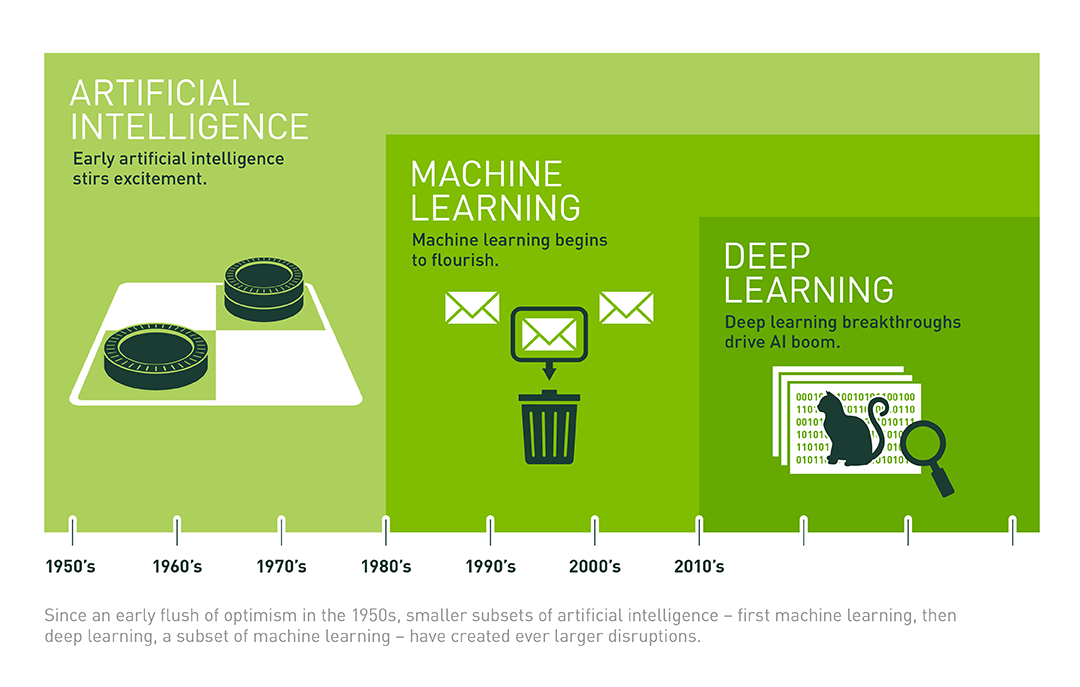
\includegraphics{evolution.png}}
	
	\end{frame}
	
	\begin{frame}[fragile,plain]
	\frametitle{Évolution de L'intelligence  Artificielle : Machine Learning}
	\begin{itemize}
		\item Le machine learning permet à une machine d’adapter ses comportements en se fondant sur l’analyse des données à sa disposition. Un robot peut ainsi apprendre à marcher en commençant par des mouvements aléatoires, puis en sélectionnant les mouvements lui permettant d’avancer.
	\end{itemize}
	\end{frame}
	
	\begin{frame}[fragile,plain]
	\frametitle{Évolution de L'intelligence  Artificielle : Deep Learning}
	\begin{itemize}
		\itemsep1em
		\item Le deep learning est la branche du machine learning qui utilise comme modèles mathématiques les réseaux de neurones formels, eux-mêmes construits sur la représentation mathématique et informatique d’un neurone biologique, née en 1943.
		\item  Le Deep Learning est utilisé dans la voiture autonome  de Google : le réseau de  neurones 	classifie tout l’environnement pour éviter les obstacles ou s’arrêter au bon moment 
	\end{itemize}
	\end{frame}
	
	\begin{frame}[fragile,plain]
	\frametitle{Évolution de L'intelligence  Artificielle}
	
	\centerline{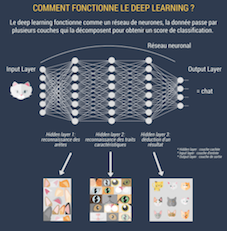
\includegraphics{deeplearning.png}}
	\end{frame}
	
		\begin{frame}[fragile,plain]
	\frametitle{Évolution de L'intelligence  Artificielle (fin)}
	\begin{itemize}
		\item Ces deux branches de l'intelligence artificielle ont causées de grandes améliorations de algorithmes, mais malgres cela l'IA d'aujourd'hui est est toujours qualifiée de « faible », en opposition à l’IA « forte » et consciente d’elle-même que prédisent les transhumanistes.

	\end{itemize}
	\end{frame}
	
	%%%%%%%%%%%%%%%%%%%%%%%%%
	%       Turing          %
	%%%%%%%%%%%%%%%%%%%%%%%%%
	
	\section{Turing et ses aboutissants}
	\begin{frame}[fragile,plain]
		\frametitle{Le Test De Turing : Définition}
		\begin{itemize}
		 \item Le test de Turing est une proposition de test d’intelligence artificielle fondée sur la faculté d'une machine à imiter la conversation humaine. Décrit par Alan Turing en 1950 dans sa publication Computing machinery and intelligence, ce test consiste à mettre un humain en confrontation verbale à l’aveugle avec un ordinateur et un autre humain \\
		 Si la personne qui engage les conversations n’est pas capable de dire lequel de ses interlocuteurs est un ordinateur, on peut considérer que le logiciel de l’ordinateur a passé avec succès le test. Cela sous-entend que l’ordinateur et l’humain essaieront d’avoir une apparence sémantique humaine.
		
		\end{itemize}
		\end{frame}
		
	\begin{frame}[fragile,plain]
		\frametitle{Schema Test De Turing}
		
		\centerline{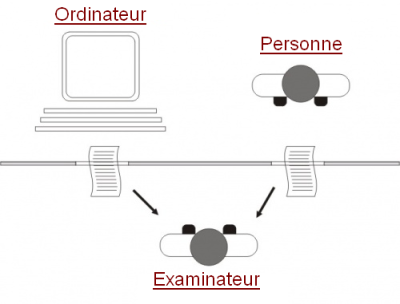
\includegraphics[scale = 0.7]{test-de-turing.png}}
	
	\end{frame}
	
	\begin{frame}[fragile,plain]
		\frametitle{Outils}
		\begin{itemize}
			\item Au cours d'une soixantaine d'années de recherche, l'IA a développé plusieurs outils pour résoudre les problèmes les plus difficiles en informatique.
			\item Recherche et Optimisation
			\item Logique
			\item Classificateurs et méthodes d'apprentissage statistique
			\item Réseaux de neurones artificiels
		\end{itemize}
	\end{frame}
	
	\begin{frame}[fragile,plain]
		\frametitle{Recherche et Optimisation}
		\begin{itemize}
		    \item Selon le scénario, il peut y avoir une ou plusieurs solutions à un problème donné, car il peut y avoir plusieurs façons de résoudre ce problème. 
		    \item Disons qu'on doit faire quelque chose comme une multiplication mathématique. Clairement, il y a une solution correcte, mais de nombreux algorithmes pour multiplier. Maintenant, prenant un problème plus compliqué, comme jouer à un jeu, Dans la plupart des cas, à un moment donné, on a plusieurs mouvements qu'on peut faire, et on choisit celui qui nous donne le meilleur résultat possible. Les agents rationnels de l'intelligence artificielle abordent les problèmes de la même manière.
		\end{itemize}
	\end{frame}
	
	
	\begin{frame}[fragile,plain]
		\frametitle{Logique}
		\begin{itemize}
		    \item La logique a joué un rôle important dans le développement de l'Intelligence Artificielle (IA). À son tour, penser à des applications dans l'IA a conduit au développement de nombreux systèmes logiques nouveaux et intéressants.
		    \item Par exemple, l'algorithme satplan utilise la logique pour la planification. Il convertit l'instance de problème de planification en une instance du problème de satisfissabilité booléenne, qui est ensuite résolue à l'aide d'une méthode permettant d'établir la satisfiabilité.
		\end{itemize}
	\end{frame}
	
	
	\begin{frame}[fragile,plain]
		\frametitle{Classificateurs et méthodes d'apprentissage statistique}
		\begin{itemize}
			\item la classification constitue une partie centrale de nombreux systèmes d'IA. 
             \item Les classificateurs sont des fonctions qui utilisent la correspondance de modèle pour déterminer la correspondance la plus proche. Un classificateur peut être formé de différentes manières; il existe de nombreuses approches statistiques et d'apprentissage automatique. L'arbre de décision est peut-être l'algorithme d'apprentissage automatique le plus utilisé.
		\end{itemize}
	\end{frame}
	
	
	\begin{frame}[fragile,plain]
		\frametitle{Réseaux de neurones artificiels}
		\begin{itemize}
		    \item  c'est un système dont la conception est à l'origine schématiquement inspirée du fonctionnement des neurones biologiques, et qui par la suite s'est rapproché des méthodes statistiques.
		    \item Les réseaux de neurones sont généralement optimisés par des méthodes d’apprentissage de type probabiliste, en particulier bayésien.dans la famille des méthodes de l’intelligence artificielle auxquelles ils fournissent un mécanisme perceptif indépendant des idées propres de l'implémenteur, et fournissant des informations d'entrée au raisonnement logique formel.
		\end{itemize}
		
	\end{frame}


	
 	\begin{frame}[fragile,plain]
 	   \frametitle{Domaines D'applications}
 	   \begin{itemize}
 	    \item Finance et L'economie
 	    \item La Sante
 	    \item L'Automobile
 	    \item Jeux Video
 	   \end{itemize}
 	\end{frame}
 	
 	
 	\begin{frame}[fragile,plain]
 	   \frametitle{Finance et L'economie}
 	        \begin{itemize}
 	            \item L'utilisation de machines IA sur le marché dans des applications telles que le commerce en ligne et la prise de décision a modifié les principales théories économiques. Par exemple, les plates-formes d'achat et de vente basées sur l'IA ont modifié la loi de l'offre et de la demande. les courbes de demande et d'offre et donc les prix individualisés
 	            
 	            \item Les banques utilisent aujourd'hui des systèmes d'intelligence artificielle pour organiser les opérations, tenir la comptabilité, investir dans les stocks et gérer les propriétés.
 	           
 	            \item L'IA a également réduit la fraude et les délits financiers en surveillant les comportements des utilisateurs en cas de changements ou d'anomalies anormaux.
 	        \end{itemize}
 	\end{frame}
 	
 	
 	\begin{frame}[fragile,plain]
 	   \frametitle{La Sante}
 	   \begin{itemize}
 	       \item des algorithmes et des logiciels sont utilisés pour approcher la cognition humaine dans l'analyse de données médicales complexes. Les programmes d'IA ont été développés et appliqués à des pratiques telles que les processus de diagnostic, le développement de protocoles de traitement, le développement de médicaments, la médecine personnalisée et la surveillance des patients, soin, entre autres.
 	       
 	       \item Par exemple ll y a une grande quantité de recherche et de médicaments développés en rapport avec le cancer. Dans le détail, il y a plus de 800 médicaments et vaccins pour traiter le cancer,et pour cela  Microsoft travaille sur un projet de développement d'une machine appelée "Hanover".
 	       
 	   \end{itemize}
 	\end{frame}
 	
 	
 		\begin{frame}[fragile,plain]
 	   \frametitle{La Sante}
 	   \begin{itemize}
 	   \item Il y a eu une étude récente réalisée par des chirurgiens du Children's National Medical Center de Washington qui a démontré avec succès la chirurgie avec un robot autonome. L'équipe a supervisé le robot pendant qu'il pratiquait une chirurgie des tissus mous, en cousant ensemble l'intestin d'un cochon pendant une chirurgie ouverte, et en le faisant mieux qu'un chirurgien humain.
 	   \end{itemize}
 	 \end{frame}
 	
 	
 	\begin{frame}[fragile,plain]
 	   \frametitle{L'Automobile}
 	   \begin{itemize}
 	       \item Les progrès de l'IA ont contribué à la croissance de l'industrie automobile grâce à la création et à l'évolution de véhicules autonomes. En 2016, plus de 30 entreprises utilisent l'IA pour la création de voitures sans conducteur. Quelques entreprises impliquées dans l'IA incluent Tesla et Google.
 	       
 	       \item De nombreux composants contribuent au fonctionnement des voitures autonomes. Ces véhicules intègrent des systèmes tels que le freinage, le changement de voie, la prévention des collisions, la navigation et la cartographie. Ensemble, ces systèmes, ainsi que les ordinateurs haute performance, sont intégrés dans un véhicule complexe.
 	   \end{itemize}
 	\end{frame}
 	
 	
 	\begin{frame}[fragile,plain]
 	   \frametitle{Jeux Video}
 	   \begin{itemize}
 	       \item Dans les jeux vidéo, l'intelligence artificielle est couramment utilisée pour générer un comportement dynamique dynamique dans les personnages non-joueurs (PNJ). De plus, des techniques d'IA bien comprises sont couramment utilisées pour le pathfinding.
 	   \end{itemize}
 	\end{frame}
	
	%%%%%%%%%%%%%%%%%%%%%%%%%
	%    Les Réalités       %
	%%%%%%%%%%%%%%%%%%%%%%%%%
	
	\section{Les Réalités}
	\begin{frame}[fragile,plain]
	\frametitle{Les Réalités de l'Intelligence Artificielle}
	\begin{block}{Les utilisations de l'IA}
	\begin{itemize}
	\itemsep1em
		\item On peut imaginer plein de possibilité avec l'utilisation de l'IA, que se soit dans :
		\begin{itemize}
		\itemsep1em
		\item L'automobile
		\item L'industriel
		\item L'armée
		\item Le médical
		\item Le jeu-vidéo
		\item La téléphonie
		\item ...
		\end{itemize}
		\end{itemize}
	\end{block}
	\end{frame}
	
	\begin{frame}[fragile,plain]
	\frametitle{Les Réalités de l'Intelligence Artificielle}
	\begin{block}{Les utilisations de l'IA}
	\begin{itemize}
	\itemsep1em
		\item De nos jours il existe plein de projets en développement et de prototypes :
		\begin{itemize}
		\itemsep1em
		\item Le SolarXOne est un drone autonome mis au point par la société Xsun et la collaboration de l’école Centrale Nantes, Dassault systèmes mais aussi Airbus. Il se recharge à l'énergie solaire et l'IA intégrée lui permet de décider, seul, de sa trajectoire en fonction de la destination mais aussi de faire attention à de différents facteurs tels que la météo.
		\item La Renault Symbioz est une voiture autonome. Elle possède 35 capteurs tout au tour d'elle. L'IA permet de conduire automatiquement sur autoroute, et passer des péages
		\item Le Robot Sophia est un robot qui possède des expressions faciales en fonction du contexte, peut répondre à des questions et enregistre les différents visages de ses interlocuteurs
		\end{itemize}
		\end{itemize}
	\end{block}
	\end{frame}
	
	\begin{frame}[fragile,plain]
	\frametitle{Les Réalités de l'Intelligence Artificielle}
	\begin{block}{Les utilisations de l'IA}
	\begin{itemize}
	\itemsep1em
		\item Dans l'industriel, les tâches répétitives ne sont plus effectuées par des humains mais par des machines programmées, ce concept est généralement adopté par les usines automobiles.
		\item Dans le médical, il existe des systèmes experts qui sont utilisés pour aider à diagnostiquer des patients.
		\item Dans le jeu-vidéo, avec l'ordinateur qui doit essayer de jouer aussi bien que l'humain pour même essayer de le battre suivant la difficulté choisie par le joueur.
		\item Dans la téléphonie, les Smartphones incorporent une multitude de programmes d'intelligence artificielle comme la reconnaissance vocale, la reconnaissance faciale ect ...
	\end{itemize}
	\end{block}
	\end{frame}
	
	%%%%%%%%%%%%%%%%%%%%%%%%%
	%     Les Promesses     %
	%%%%%%%%%%%%%%%%%%%%%%%%%
	
	\section{Les Promesses}
	\begin{frame}[fragile,plain]
	\frametitle{Les Promesses de l'Intelligence Artificielle}
	\begin{block}{L'avenir de l'IA}
	\begin{itemize}
	\itemsep1em
		\item Le future de l'IA pourrait, dans les différents domaines évoqués au-dessus, améliorer la vie des Hommes, la rendre mieux et la faciliter
		\item En médecine, il se pourrait que des machines, robots nous opèrent, nous diagnostiquent, ce qui enlèverait le facteur Humain, c'est-à-dire fire des erreurs dans une opération ou dans un diagnostique
		\item Avec les drones, on se penche sur des drones qui pourraient aider l'homme dans des domaines différents, telle que le sauvetage, la cartographie 3D, l'armée, sur le marché de la surveillance des infrastructures et réseaux qui requièrent un monitoring récurrent, %comme les pipelines, les lignes ferrovaires et électriques... 
		des usages sont aussi imaginés pour la surveillance du trafic, de la pollution ou l'agriculture de précision
	\end{itemize}
	\end{block}
	\end{frame}	
	
	\begin{frame}[fragile,plain]
	\frametitle{Les Promesses de l'Intelligence Artificielle}
	\begin{block}{L'avenir de l'IA}
	\begin{itemize}
	\itemsep1em
		\item Des robots comme Kenshiro et kengoro devraient permettre, à terme, de mieux comprendre le corps humain et ses mouvements, "encore trop incompris" ou encore pouvoir aider l'Homme dans des tâches quotidienne (nettoyage, rangements...). Ils peuvent être utiles aussi dans l'armée
		\item Airbus et Audi, sont en train de travailler sur un projet de véhicule à la fois terrestre et volant nommé Pop.Up
	\end{itemize}
	\end{block}
	\end{frame}
	
	%%%%%%%%%%%%%%%%%%%%%%%%%
	%     Les Dangers       %
	%%%%%%%%%%%%%%%%%%%%%%%%%
	
	\section{Les Dangers}
	\begin{frame}[fragile,plain]
	\frametitle{Les Dangers de l'Intelligence Artificielle}
	\begin{block}{Les inquiétudes sur l'IA}
	\begin{itemize}
	\itemsep1em
		\item En 2014, Stephen Hawking met en garde sur le risque que l'IA devienne plus intelligente que l'Homme et le domine
		\item Moshe Vardi, un spécialiste américain de l'informatique, suppose que l'IA pourrait mettre 50\% de l'humanité au chômage
		\item En Février 2018, 26 experts spécialistes en intelligence artificielle mettent en garde contre les dangers d'un usage criminelle de l'IA : augmentation de la la cybercriminalité , conduire à des utilisations de drones ou de robots à des fins terroristes, etc...
		\item Selon eux, dans les dix prochaines années, l'efficacité croissante de l'IA risque de renforcer la cybercriminalité mais aussi de conduire à des utilisations de drones ou de robots à des fins terroristes
		\end{itemize}
	\end{block}
	\end{frame}

	\begin{frame}[fragile,plain]
	\frametitle{Les Dangers de l'Intelligence Artificielle}
	\framesubtitle{Google Home}
	\centerline{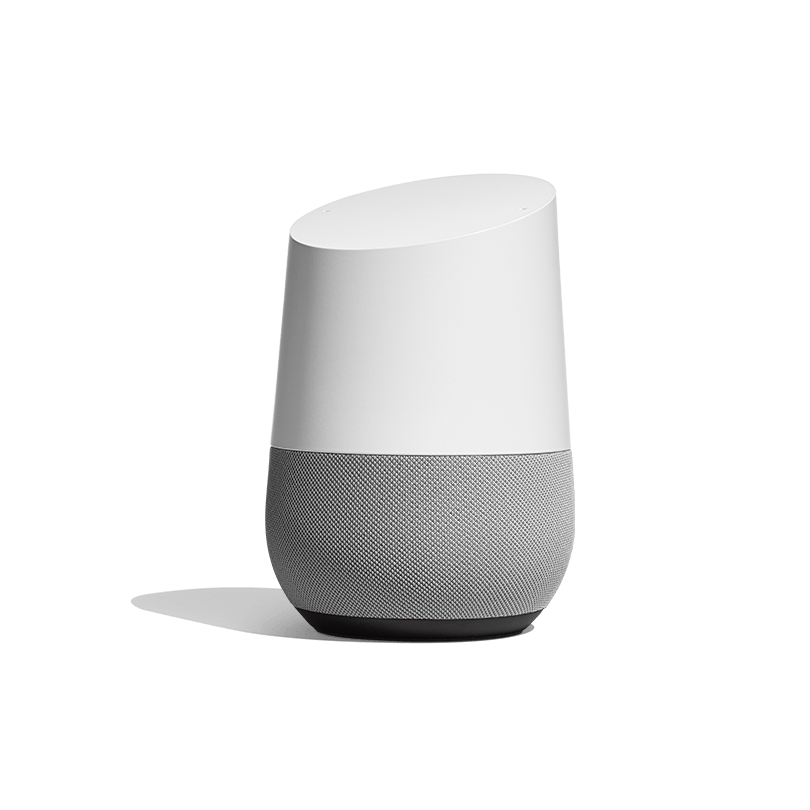
\includegraphics[height=8cm]{googlehome.png}}
	\end{frame}
	
	\begin{frame}[fragile,plain]
	\frametitle{Les Dangers de l'Intelligence Artificielle}
	\framesubtitle{Google Home}
	\begin{block}{Google Home}
	\begin{itemize}
	\itemsep1em
		\item Le Google Assistant est une IA inclus dans le Google Home
		\item On peut lui poser toutes sortes de questions ou lui demander des services (Planifier votre journée, Contrôler votre maison connectée, Gérer les tâches...)
		\item Toutes actions sur le Google Home est enregistré et peut-être détourné de façon commerciale ou malveillante
	\end{itemize}
	\end{block}
	\end{frame}
	
	\begin{frame}[fragile,plain]
	\frametitle{Les Dangers de l'Intelligence Artificielle}
	\framesubtitle{Drones Autonomes}
	\centerline{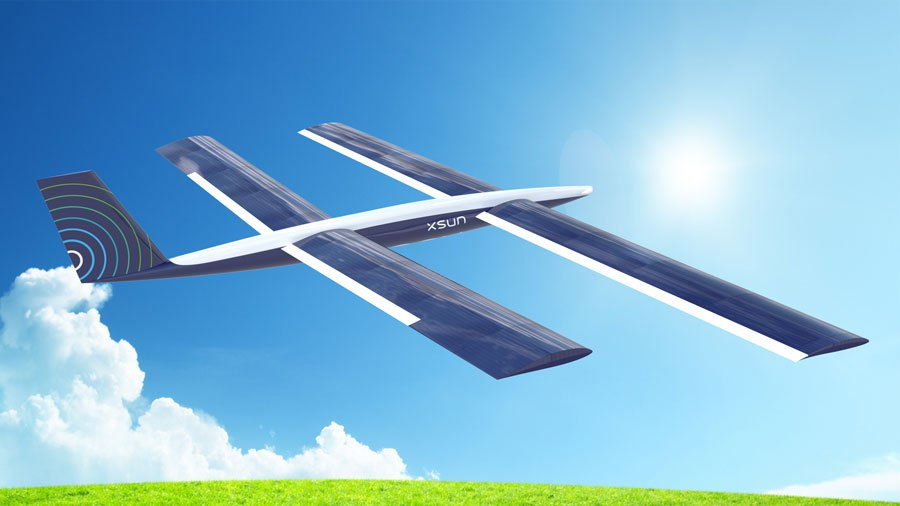
\includegraphics[height=6cm]{drone.jpg}}
	\end{frame}
	
	\begin{frame}[fragile,plain]
	\frametitle{Les Dangers de l'Intelligence Artificielle}
	\framesubtitle{Drones Autonomes}
	\begin{block}{Drones Autonomes}
	\begin{itemize}
	\itemsep1em
		\item La Nasa dévoloppe des Drones Autonomes utilisant la technologie de Google nommé Tango qui permet de faire une cartographie 3D en temps réel
		\item Pour la Nasa, et Google, le principal intérêt de cette expérimentation est d'utiliser la Technologie Tango en alternative au GPS pour évoluer à l'intérieur des bâtiments. Cette technologie pourrait se retrouver un jour sur des drones ou des robots amenés à travailler dans des entrepôts ou à évoluer sur des zones sinistrées lors de missions de sauvetage
		\item Des Drones Autonomes pourraient servir d'armes pour l'Armée. La CCAC (Convention sur certaines armes classiques) n'ont pas abouti à des décisions concrètes sur l'utilisation des Drones Autonomes
	\end{itemize}
	\end{block}
	\end{frame}
	
	\begin{frame}[fragile,plain]
	\frametitle{Les Dangers de l'Intelligence Artificielle}
	\framesubtitle{Voitures Autonomes}
	\centerline{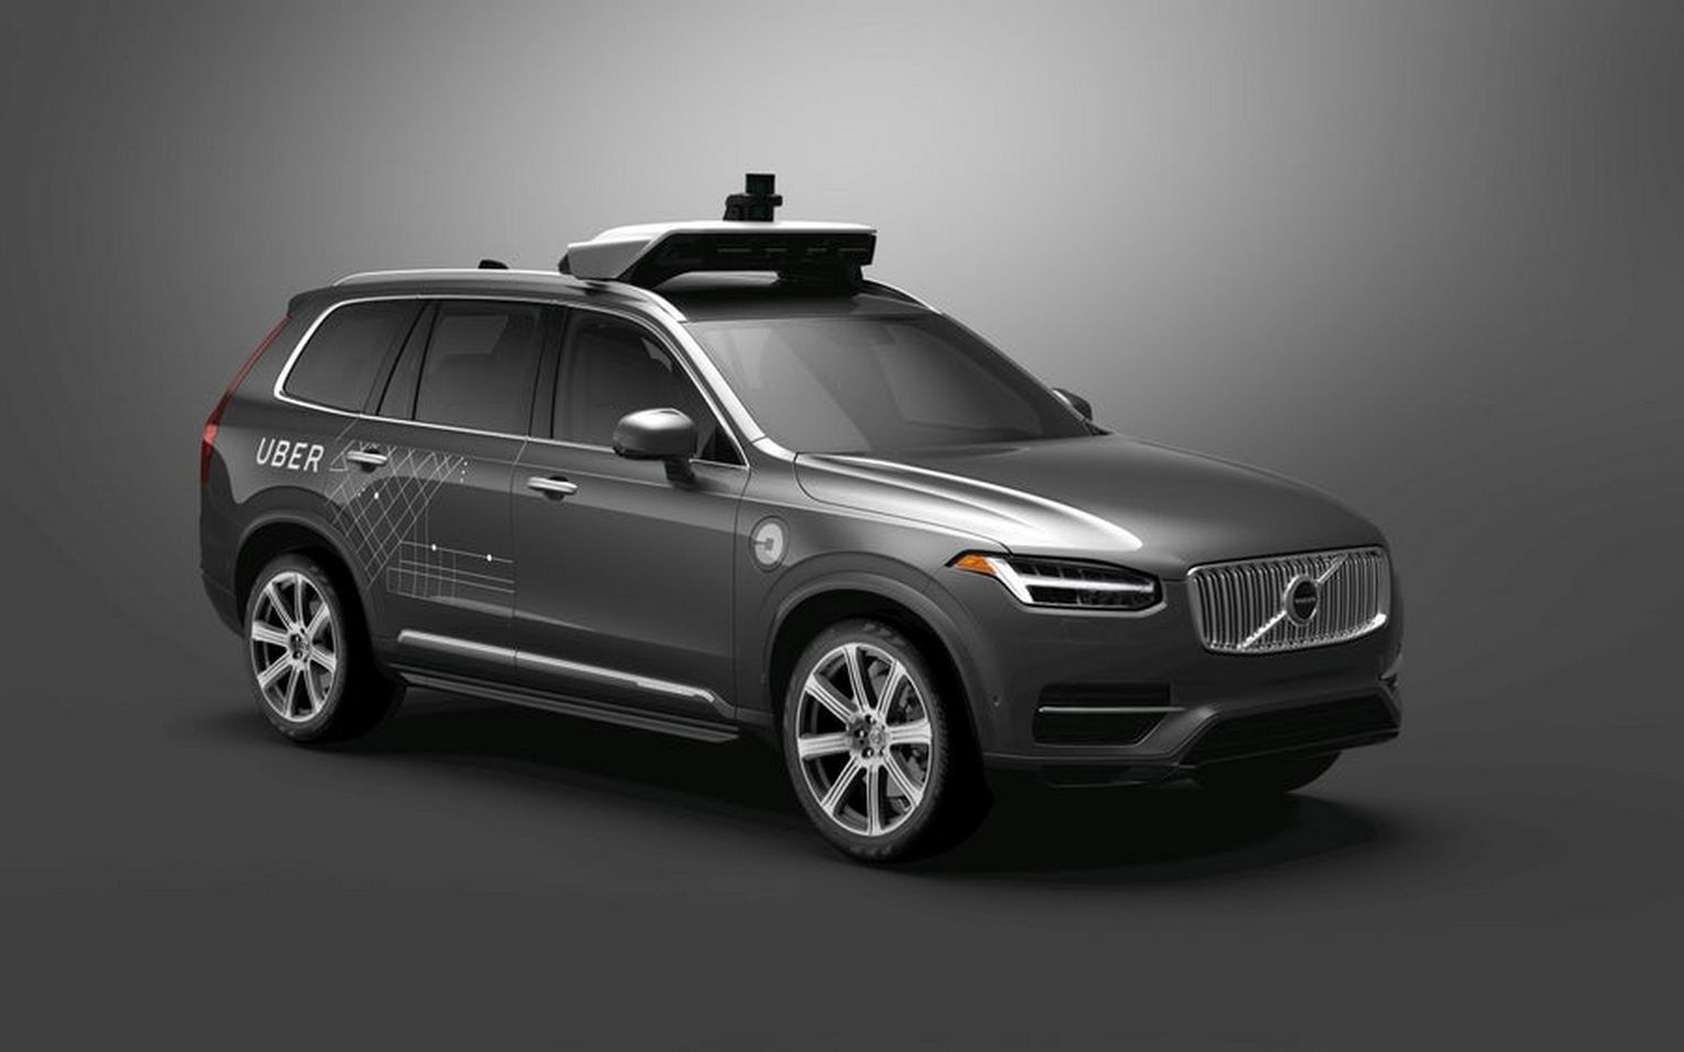
\includegraphics[height=6cm]{uber.jpg}}
	\end{frame}
	
	\begin{frame}[fragile,plain]
	\frametitle{Les Dangers de l'Intelligence Artificielle}
	\framesubtitle{Voitures Autonomes}
	\begin{block}{Voitures Autonomes}
	\begin{itemize}
	\itemsep1em
		\item Les voitures autonomes sont conçus pour être conduite par une IA
		\item La sécurité est le point le plus important et ce n'est pas toujours parfait
		\item Le 19 Mars 2018, un accident mortel entre une voiture autonome et un piéton
		\item Le MIT (Massachusetts Institute of Technology) ont développé un test nommé Moral Machine pour tester les humains sur des questions morales
	\end{itemize}
	\end{block}
	\end{frame}
	
	\begin{frame}[fragile,plain]
	\frametitle{Les Dangers de l'Intelligence Artificielle}
	\framesubtitle{Voitures Autonomes}
	\centerline{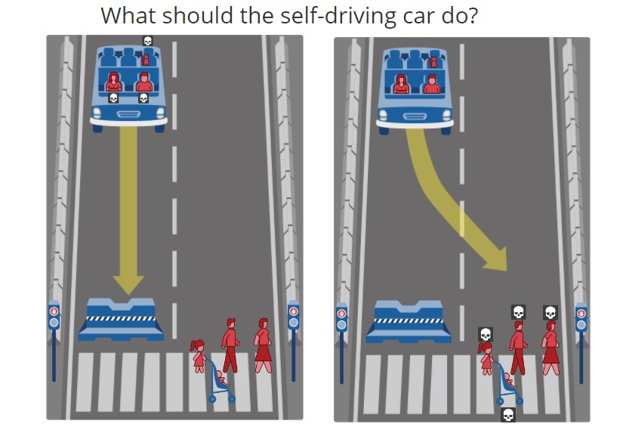
\includegraphics[height=6cm]{MIT.jpg}}
	\end{frame}
	
	\begin{frame}[fragile,plain]
	\frametitle{Les Dangers de l'Intelligence Artificielle}
	\framesubtitle{Voitures Autonomes}
	\centerline{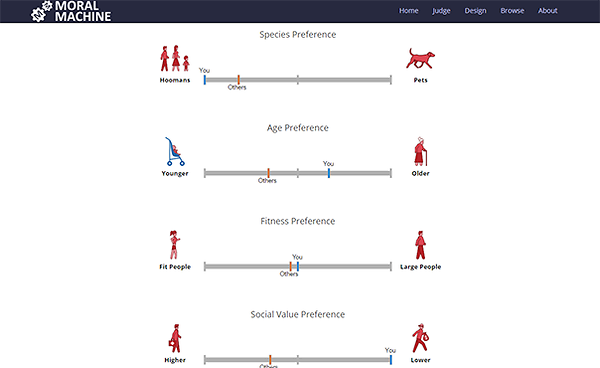
\includegraphics[height=6cm]{MIT2.png}}
	\end{frame}
	
	\begin{frame}[fragile,plain]
	\frametitle{Les Dangers de l'Intelligence Artificielle}
	\framesubtitle{Robots, Humanoïdes}
	\centerline{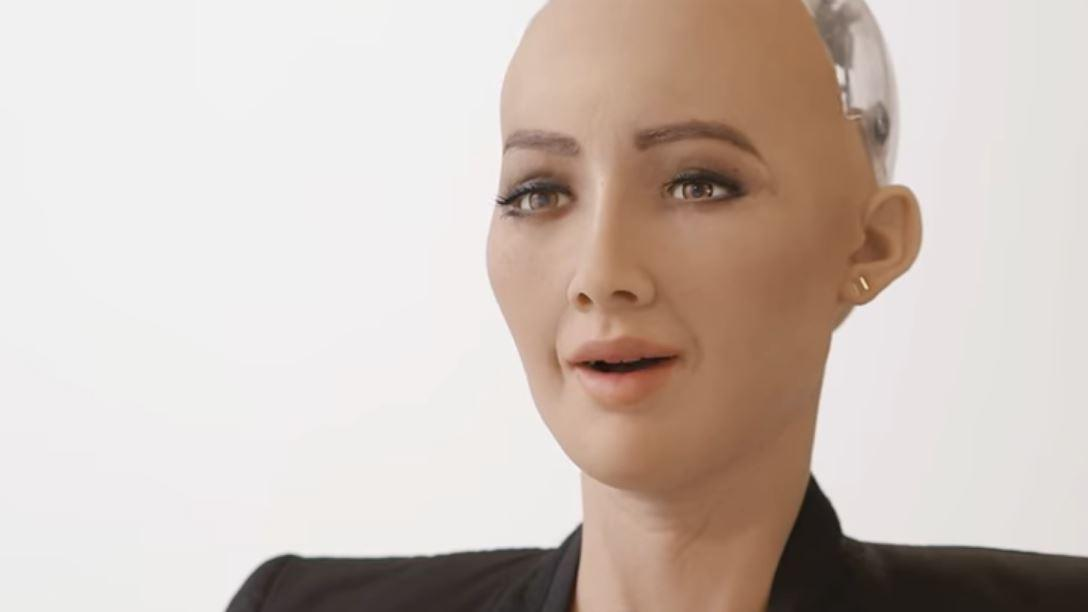
\includegraphics[height=6cm]{robotSophia.jpeg}}
	\end{frame}
	
	\begin{frame}[fragile,plain]
	\frametitle{Les Dangers de l'Intelligence Artificielle}
	\framesubtitle{Robots, Humanoïdes}
	\centerline{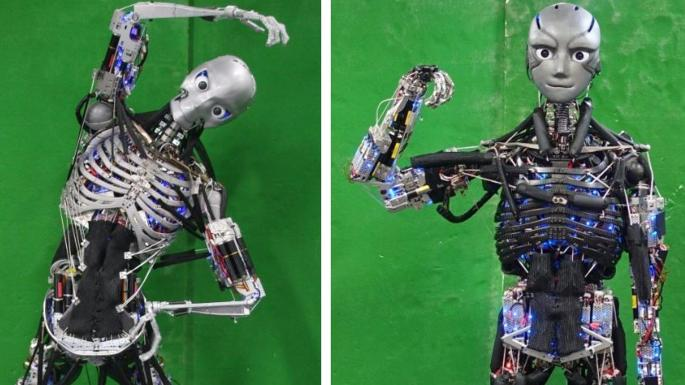
\includegraphics[height=6cm]{kenshiro_kengoro.jpg}}
	\end{frame}
	
	\begin{frame}[fragile,plain]
	\frametitle{Les Dangers de l'Intelligence Artificielle}
	\framesubtitle{Robots, Humanoïdes}
	\begin{block}{Robots, Humanoïdes}
	\begin{itemize}
	\itemsep1em
		\item Isaac Asimov a créé les 3 lois de la Robotique :
		\begin{itemize}
		\itemsep1em
			\item Première loi : Un robot ne peut porter atteinte à un être humain ni, restant passif, laisser cet être humain exposé au danger.
			\item Deuxième loi : Un robot doit obéir aux ordres donnés par les êtres humains, sauf si de tels ordres sont en contradiction avec la première loi.
			\item Troisième loi : Un robot doit protéger son existence dans la mesure ou cette protection n'est pas en contradiction avec la première ou la deuxième loi.
		\end{itemize}
		\item Beaucoup de films traitent le sujet des dangers avec les Humanoïdes
	\end{itemize}
	\end{block}
	\end{frame}
	
	%%%%%%%%%%%%%%%%%%%%%%%%%
	%       Annexes         %
	%%%%%%%%%%%%%%%%%%%%%%%%%	
	
	\section{Annexes}
	\begin{frame}[fragile,plain]
	\frametitle{Annexes}
	\begin{itemize}
	\itemsep1em
		\item Les Réalités :
		\begin{itemize}
		\itemsep1em
			\item https://www.lesnumeriques.com/voiture/renault-symbioz-demo-voiture-autonome-niveau-4-est-realite-a3433.html
			\item https://www.sciencesetavenir.fr/high-tech/intelligence-artificielle/sophia-le-robot-de-hanson-robotics-qui-va-vous-faire-peur\_103728
			\item http://tpeai.e-monsite.com/pages/i-l-etat-de-l-intelligence-artificielle-aujourd-hui.html
		\end{itemize}
		\end{itemize}
	\end{frame}	
		
	\begin{frame}[fragile,plain]
	\frametitle{Annexes}
	\begin{itemize}
	\itemsep1em
		\item Les Dangers
		\begin{itemize}
		\itemsep1em
			\item https://fr.wikipedia.org/wiki/Intelligence\_artificielle
			\item https://www.cnas.org/publications/reports/malicious-ai-report
			\item https://www.lesechos.fr/tech-medias/hightech/0301328931624-intelligence-artificielle-un-rapport-pointe-les-risques-dune-utilisation-criminelle-2155398.php
			\item https://www.sciencesetavenir.fr/high-tech/transports/accident-mortel-entre-un-pieton-et-une-voiture-autonome-uber-la-police-publie-la-video\_122190
			\item https://www.lesechos.fr/industrie-services/automobile/0301463184693-conducteur-contre-pieton-les-dilemmes-vertigineux-de-la-voiture-autonome-2163847.php
%			\item https://start.lesechos.fr/actu-entreprises/industries/voiture-autonome-le-test-ethique-du-mit-pour-decider-qui-sauver-5897.php
			\item https://en.wikipedia.org/wiki/Moral\_Machine
			\item http://www.phonandroid.com/google-home-amazon-echo-cnil-alerte-utilisateurs-dangers-lies-a-vie-privee.html
			\item http://www.frandroid.com/produits-android/accessoires-objets-connectes/454464\_a-quoi-sert-le-google-home-lenceinte-intelligente-et-assistant-pour-la-maison
			\item https://www.futura-sciences.com/tech/actualites/drone-course-drones-ia-nasa-mesure-pilote-humain-69368/
			\item https://fr.wikipedia.org/wiki/Convention\_sur\_certaines\_armes\_classiques\#\%C3\%89volutions\_r\%C3\%A9centes
			\item https://siecledigital.fr/2016/06/10/google-tango-lenovo/
			\item https://www.sciencesetavenir.fr/high-tech/robot/ia-et-robot-citoyen-en-arabie-saoudite-un-bluff-dangereux-selon-laurence-devillers\_117933
			\item https://www.lexpress.fr/actualite/sciences/video-kengoro-le-robot-ultra-perfectionne-qui-transpire-quand-il-fait-des-pompes\_1972852.html
		\end{itemize}
		\end{itemize}
	\end{frame}
	
	\begin{frame}[fragile,plain]
	\frametitle{Annexes}
	\begin{itemize}
	\itemsep1em
		\item https://start.lesechos.fr/actu-entreprises/industries/voiture-autonome-le-test-ethique-du-mit-pour-decider-qui-sauver-5897.php
		\item https://en.wikipedia.org/wiki/Moral\_Machine
		\item http://www.phonandroid.com/google-home-amazon-echo-cnil-alerte-utilisateurs-dangers-lies-a-vie-privee.html
		\item http://www.frandroid.com/produits-android/accessoires-objets-connectes/454464\_a-quoi-sert-le-google-home-lenceinte-intelligente-et-assistant-pour-la-maison
		\item https://www.futura-sciences.com/tech/actualites/drone-course-drones-ia-nasa-mesure-pilote-humain-69368/
	\end{itemize}
	\end{frame}
	
		\begin{frame}[fragile,plain]
	\frametitle{Annexes}
	\begin{itemize}
	\itemsep1em
		\item https://fr.wikipedia.org/wiki/Convention\_sur\_certaines\_armes\\
		\_classiques\#\%C3\%89volutions\_r\%C3\%A9centes
		\item https://siecledigital.fr/2016/06/10/google-tango-lenovo/
		\item https://www.sciencesetavenir.fr/high-tech/robot/ia-et-robot-citoyen-en-arabie-saoudite-un-bluff-dangereux-selon-laurence-devillers\_117933
		\item https://www.lexpress.fr/actualite/sciences/video-kengoro-le-robot-ultra-perfectionne-qui-transpire-quand-il-fait-des-pompes\_1972852.html
	\end{itemize}
	\end{frame}
	
\end{document}